\section{METHODOLOGY}
\label{sec:methodology}

We describe the implemented pipeline first
(Sections~\ref{subsec:method-overview}--\ref{subsec:method-render}) and then
the stage-level evaluations used to test the hypotheses
(Section~\ref{subsec:method-eval}).

\subsection{System Overview}
\label{subsec:method-overview}

The system processes each PDF through three stages connected by a single JSON
intermediate representation (Figure~\ref{fig:pipeline-overview}). This separation
is methodological as well as
engineering: H1 asks which stage binds quality, so the parser, translator and
reconstructor must each expose an output that can be inspected and scored.

\begin{figure}[tb]
    \centering
    
\includegraphics[width=0.9\textwidth]{overview_architect.png}
    \caption{The three-stage pipeline. Each stage consumes the previous
    artifact and writes a new JSON/PDF artifact into a per-session working
    directory, so individual stages can be inspected, corrected or re-run.}
    \label{fig:pipeline-overview}
\end{figure}

\begin{description}[leftmargin=0em,labelsep=0.4em]
  \item[Stage~1 --- Structure analysis.] The source PDF is rendered page by page
  and analysed visually. The output is a \texttt{ParsedDocument} whose elements
  carry page index, bounding box, type label, OCR text, reading order and, for
  tables, cell boxes.
  \item[Stage~2 --- Content translation.] Translatable elements are packed in
  document order and translated by an LLM under an identifier-preserving
  contract, with dedicated handling for tables, formulas and terminology.
  \item[Stage~3 --- Reconstruction.] Translated strings are placed back on the
  source page. Font size is decided from source geometry and local collisions;
  background and text colour are estimated from source pixels before the overlay
  is composited onto the original PDF.
\end{description}

\paragraph{Human-in-the-loop checkpoints.} The prototype exposes two optional
checkpoints: after Stage~1, users can correct labels, OCR text, bypass flags and
table-cell text; after Stage~3, they can edit text on the rendered page. These
checkpoints are not included in the automatic evaluation, but they target the
same unrecoverable errors analysed in Section~\ref{sec:results}.

\subsection{Stage 1: Document Structure Analysis}
\label{subsec:method-parser}

The parser deliberately ignores the embedded text layer and treats every page as
an image. This gives one path for born-digital, scanned and mixed PDFs, avoiding
the common failure in which a hidden OCR layer or broken font encoding differs
from what the reader sees.

\subsubsection{Models and Output Representation}

Four models are used in three modules. Surya Layout predicts page regions and
labels; Surya Text Detection localises text lines; Surya Text Recognition reads
their content; and a PaddleOCR RT-DETR table-cell detector identifies cell boxes
inside table regions~\citep{surya,paddleocr}; detected cell boxes are kept as
geometry for cell-wise translation (Figure~\ref{fig:table-cells}). OCR is run before layout
post-processing so its line boxes can tighten regions, split sparse blocks and
recover missed text (Figure~\ref{fig:parser-stages}).

\begin{figure}[H]
  \centering
  \begin{subfigure}[t]{0.25\textwidth}
    \centering
    
\includegraphics[width=\linewidth]{ocr_page12_original.png}
    \caption{Source page}
  \end{subfigure}\hfill
  \begin{subfigure}[t]{0.25\textwidth}
    \centering
    
\includegraphics[width=\linewidth]{ocr_page12_detection.png}
    \caption{Text detection}
  \end{subfigure}\hfill
  \begin{subfigure}[t]{0.25\textwidth}
    \centering
    
\includegraphics[width=\linewidth]{ocr_page12_recognition.png}
    \caption{Text recognition}
  \end{subfigure}\hfill
  \begin{subfigure}[t]{0.25\textwidth}
    \centering
    
\includegraphics[width=\linewidth]{layout_page12.png}
    \caption{Layout detection}
  \end{subfigure}
  \caption{Page-level recognition stages: (a) the rasterised page is the input;
  (b) individual text lines are localised; (c) each line is recognised and
  re-anchored to its position; (d) the layout model delimits blocks, coloured by
  coarse \texttt{category} and labelled with the fine-grained class.}
  \label{fig:parser-stages}
\end{figure}

\begin{figure}[H]
  \centering
  
\includegraphics[width=0.4\linewidth]{table_cells_page12.png}
  \caption{Table-cell detection: the PaddleOCR RT-DETR detector returns a box per
  cell inside each table region; the boxes are kept as geometry for cell-wise
  translation and table reconstruction.}
  \label{fig:table-cells}
\end{figure}

The resulting \texttt{ParsedDocument} is a tree of pages and elements. Each
\texttt{ElementData} stores the fine label, coarse category, PDF-space bounding
box and source text. Table elements additionally store a flat list of cells,
each with a grid box and a tight text box. The fine labels are mapped to four
translation policies:

\begin{itemize}[leftmargin=1.2em]
  \item \texttt{FLOWING\_TEXT}: paragraphs, lists, captions, footnotes, section
  headers, forms and tables of contents; translated as text and re-wrapped.
  \item \texttt{TABLE}: translated cell by cell so content remains tied to its
  original cell geometry.
  \item \texttt{EQUATION}: isolated formula regions; preserved or processed by
  the formula-specific path.
  \item \texttt{BYPASS}: figures, pictures, code, page headers and footers;
  copied from the source page without translation.
\end{itemize}

\subsubsection{Translation-Oriented Post-processing}

Detected OCR lines are assigned to a layout block when at least $50\%$ of the
line area lies inside it, then sorted by row and $x$ position. Text is normalised
to NFC, control characters are removed except newline and tab, whitespace is
collapsed, and empty outer lines are trimmed.

Three repairs make the output useful for translation rather than plain
extraction. \texttt{BYPASS} blocks are kept as image regions. Sparse blocks are
split when formula regions contain multiple OCR lines or when wide intra-row
gaps reveal unrelated text clusters (Figure~\ref{fig:sparse-split}). Reading
order is repaired by expanding boxes over overlapping OCR lines (coverage
$\ge0.3$), pruning nested duplicates (containment $\ge0.7$) and promoting
unassigned OCR lines to \texttt{Text} (Figure~\ref{fig:reading-order}). These
steps never invent content; they
only attach existing OCR lines to geometric elements before translation.

\begin{figure}[H]
  \centering
  \begin{subfigure}[t]{0.47\textwidth}
    \centering
    
\includegraphics[width=0.8\linewidth]{layout_calculus_p2_before.png}
    \caption{Before splitting}
  \end{subfigure}\hfill
  \begin{subfigure}[t]{0.47\textwidth}
    \centering
    
\includegraphics[width=0.8\linewidth]{layout_calculus_p2_after.png}
    \caption{After splitting}
  \end{subfigure}
  \caption{Sparse-block splitting separates formula-heavy regions into
  translatable line-level elements while preserving bypassed regions.}
  \label{fig:sparse-split}
\end{figure}

\begin{figure}[H]
  \centering
  \tikzset{
    blk/.style={draw, line width=0.6pt},
    tline/.style={draw=gray!55, fill=gray!22, line width=0.2pt},
    hot/.style={draw=red!80, fill=red!10, line width=0.5pt, dashed},
    hoton/.style={draw=red!80, fill=red!12, line width=0.5pt},
    ghost/.style={draw=gray!55, line width=0.5pt, dashed},
    lbl/.style={font=\scriptsize},
    tag/.style={font=\tiny\itshape, gray!55!black},
    num/.style={font=\scriptsize\bfseries, fill=white, inner sep=1pt},
    flow/.style={-{Latex}, line width=0.7pt},
  }
  \begin{subfigure}[t]{0.32\textwidth}\centering
  \begin{tikzpicture}[scale=0.85, transform shape]
    \draw[blk] (0,0) rectangle (2.2,1.4);
    \fill[tline] (0.2,1.02) rectangle (2.0,1.22);
    \fill[tline] (0.2,0.60) rectangle (2.0,0.80);
    \draw[hot]   (0.2,-0.22) rectangle (2.0,0.10);
    \node[tag] at (1.1,-0.5) {tight box, line spills};
    \draw[flow] (2.55,0.5) -- (3.25,0.5) node[midway,above,font=\tiny]{$\ge0.3$};
    \begin{scope}[xshift=3.6cm]
      \draw[blk] (0,-0.30) rectangle (2.2,1.4);
      \fill[tline] (0.2,1.02) rectangle (2.0,1.22);
      \fill[tline] (0.2,0.60) rectangle (2.0,0.80);
      \fill[hoton] (0.2,-0.18) rectangle (2.0,0.14);
      \node[tag] at (1.1,-0.55) {box hugs glyphs};
    \end{scope}
  \end{tikzpicture}
  \caption{Boundary expansion}
  \end{subfigure}\hfill
  \begin{subfigure}[t]{0.32\textwidth}\centering
  \begin{tikzpicture}[scale=0.85, transform shape]
    \draw[blk] (0,0.15) rectangle (2.2,1.4);
    \draw[hot] (0.28,0.42) rectangle (1.5,1.15);
    \draw[blk] (0,-0.95) rectangle (2.2,-0.15);
    \node[tag] at (1.1,-1.3) {contained in larger};
    \draw[flow] (2.55,0.2) -- (3.25,0.2) node[midway,above,font=\tiny]{$\ge0.7$};
    \begin{scope}[xshift=3.6cm]
      \draw[blk] (0,0.15) rectangle (2.2,1.4);
      \draw[ghost] (0.28,0.42) rectangle (1.5,1.15);
      \draw[red!80, line width=0.5pt] (0.28,0.42)--(1.5,1.15) (0.28,1.15)--(1.5,0.42);
      \draw[blk] (0,-0.95) rectangle (2.2,-0.15);
      \node[num] at (0.32,1.08) {1};
      \node[num] at (0.32,-0.55) {2};
      \node[tag] at (1.1,-1.3) {pruned, re-sorted};
    \end{scope}
  \end{tikzpicture}
  \caption{Containment pruning}
  \end{subfigure}\hfill
  \begin{subfigure}[t]{0.32\textwidth}\centering
  \begin{tikzpicture}[scale=0.85, transform shape]
    \draw[blk] (0,0.75) rectangle (2.2,1.45);
    \node[num] at (0.32,1.10) {1};
    \draw[hot] (0.2,0.28) rectangle (2.0,0.56);
    \node[tag, red!70!black] at (1.1,0.1) {orphan (no block)};
    \draw[blk] (0,-0.85) rectangle (2.2,-0.35);
    \node[num] at (0.32,-0.60) {2};
    \draw[flow] (2.55,0.4) -- (3.25,0.4) node[midway,above,font=\tiny]{promote};
    \begin{scope}[xshift=3.6cm]
      \draw[blk] (0,0.75) rectangle (2.2,1.45);
      \node[num] at (0.32,1.10) {1};
      \draw[blk] (0,0.20) rectangle (2.2,0.62);
      \node[num] at (0.32,0.41) {2};
      \node[lbl] at (1.35,0.41) {\texttt{Text}};
      \draw[blk] (0,-0.85) rectangle (2.2,-0.35);
      \node[num] at (0.32,-0.60) {3};
      \node[tag] at (1.1,-1.15) {inserted in order};
    \end{scope}
  \end{tikzpicture}
  \caption{Orphan-line insertion}
  \end{subfigure}
  \caption{Reading-order repair (before $\rightarrow$ after; solid black = layout
  block, grey = OCR text line, red dashed = affected element). (a) OCR lines
  overlapping a block by at least $0.3$ are absorbed and the block expands to hug
  the glyphs. (b) A block is removed when $\ge 0.7$ of its area lies inside a
  larger retained block, and the rest are re-sorted by position. (c) An OCR line
  covered by no block becomes a \texttt{Text} element inserted at the right
  position in the reading sequence.}
  \label{fig:reading-order}
\end{figure}

For tables, the parser keeps detected cells as a flat coordinate list rather
than inferring a full HTML tree. This is enough
for cell-wise translation and
grid reconstruction while avoiding brittle table-structure inference. Pages are
rasterised at two resolutions: a standard resolution for layout and detection,
and a higher one for text recognition, which is the part most sensitive to small
or blurred glyphs.

\subsection{Stage 2: Content Translation}
\label{subsec:method-translate}

This stage translates the source text of the \texttt{ParsedDocument}. Its main
task is preserving the link between content and geometry across model calls:
every translated string must return to the element or cell it came from, and
non-textual structure must stay addressable.

\subsubsection{Translation Units and Prompt Contract}
\label{subsubsec:prompt}

Each translatable element becomes one unit; table cells become separate units;
formula blocks are routed through the path in Section~\ref{subsubsec:special}.
Units are packed into bounded chunks in document order, giving the model local
context while keeping responses small enough to validate.

The central contract is an identifier bijection: every input unit identifier
must appear exactly once in the model output. The prompt also injects
document-level glossary entries relevant to the chunk, preserves URLs,
placeholders, tags and mathematical expressions, requests Typst-compatible math
inside \texttt{<math>...</math>}, and states the $\pm15\%$ character-length
preference evaluated later. Semantic adequacy is prioritised above that length
preference.

Outputs are accepted only after identifier and content validation. If the
identifier contract fails, only the affected units are requested again; if
repair still fails, the source string is kept and the event is logged so no
region is left empty in the final PDF.

\subsubsection{Handling Tables and Formulas}
\label{subsubsec:special}

Tables and formulas bypass the ordinary text path. For tables, the dominant risk
is OCR corruption: a single wrong digit or symbol can invalidate a row. Before
translation, the system crops the table from the source page and asks a
multimodal model to verify the per-cell OCR; returned corrections overwrite the
OCR data before cell-wise translation.

For formulas, the difficult case is a block that mixes prose and notation. Pure
formula regions are skipped; mixed regions are cropped and sent to a vision
model that translates the prose while preserving the mathematics, wrapped in the
\texttt{<math>} syntax required by reconstruction.

\subsubsection{Format Post-processing}

After all segments are translated, two cross-segment structures are repaired.
Tables of contents are reshaped into \verb|"<title>\t<page>"| lines when
per-line translation collapses dot leaders. Residual formulas in ordinary text
are detected from LaTeX commands, Greek symbols and super/subscript syntax, then
re-wrapped or converted to valid \texttt{<math>} Typst syntax. Invalid repairs
are rejected and the previous renderable translation is kept.

\subsection{Stage 3: Document Reconstruction}
\label{subsec:method-render}

Reconstruction is where H2 is enforced. The translator has strings but not the
page: it cannot know which neighbour a block would collide with, which font size
preserves the page hierarchy, or what colour should cover and replace the source
glyphs. The reconstruction stage therefore owns geometry and appearance.

\subsubsection{Size Selection}
\label{subsubsec:sizing}

For a text string and a box, the primitive operation is \texttt{autofit}: binary
search for the largest font size whose wrapped text fits the box height. The
pipeline does not simply use that value on each translated block. Instead, it
groups same-role elements, computes \texttt{autofit} on their \emph{source} text,
clusters the source sizes in one dimension, and uses the cluster median as the
canonical size for that role. This preserves the source document's typographic
hierarchy.

Translated text departs from the canonical size only when necessary
(Figure~\ref{fig:overflow-collision}). If it fits, the canonical size is kept.
If it overflows into local free space, the canonical size is still kept and only
the typesetting frame is extended. A block is shrunk toward its translated
\texttt{autofit} only when the overflow intersects a neighbouring retained
element. The experiments use fixed parameters for clustering, the 7~pt
readability floor, the 80~pt expansion cap and the table-cell scale factor
(Appendix~\ref{app:implementation}).

\begin{figure}[H]
    \centering
    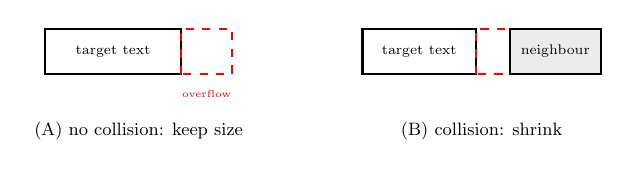
\begin{tikzpicture}[scale=0.72, transform shape]
        \begin{scope}
            \draw[thick] (0,0) rectangle (2.4,0.8);
            \node[font=\scriptsize] at (1.2,0.4) {target text};
            \draw[dashed, thick, red] (2.4,0) rectangle (3.3,0.8);
            \node[font=\tiny, red] at (2.85,-0.35) {overflow};
            \node[font=\small] at (1.65,-1.0) {(A) no collision: keep size};
        \end{scope}
        \begin{scope}[xshift=5.6cm]
            \draw[thick] (0,0) rectangle (2.0,0.8);
            \node[font=\scriptsize] at (1.0,0.4) {target text};
            \draw[dashed, thick, red] (2.0,0) rectangle (2.9,0.8);
            \draw[thick, fill=gray!15] (2.6,0) rectangle (4.2,0.8);
            \node[font=\scriptsize] at (3.4,0.4) {neighbour};
            \node[font=\small] at (2.1,-1.0) {(B) collision: shrink};
        \end{scope}
    \end{tikzpicture}
    \vspace{0.4em}
    \caption{Font size changes only when rendered overflow would collide with a
    neighbouring element.}
    \label{fig:overflow-collision}
\end{figure}

\subsubsection{Colour Selection}
\label{subsubsec:colour}

Two colours must be inferred for each translated element: the background used to
mask the source text and the colour used to draw the target text. Neither is
available uniformly from the PDF content stream, so both are sampled from the
rendered page (Figure~\ref{fig:colour-sampling}). Background colour comes from a
6~pt ring around the element at $2\times$ raster scale; contaminated light rings
are trimmed before taking a per-channel median. Text colour comes from the
central $60\%$ of the box: pixels whose RGB distance from the background exceeds
80 are glyph candidates, and the foreground is the median of the furthest half.
The rule is orientation-free, so it works for dark-on-light, light-on-dark and
saturated slide text. Textured backgrounds and boxes whose centre is mostly
whitespace remain expected failure cases.

\begin{figure}[H]
    \centering
    \begin{tikzpicture}[scale=0.7, transform shape]
        \fill[gray!30] (-0.4,-0.4) rectangle (6.4,2.2);
        \fill[white]   (0,0)       rectangle (6,1.8);
        \draw[dashed]  (-0.4,-0.4) rectangle (6.4,2.2);
        \draw[thick]   (0,0)       rectangle (6,1.8);
        \draw[dotted, thick] (1.2,0.36) rectangle (4.8,1.44);
        \node[font=\scriptsize] at (3,0.9) {source glyphs};
        \node[font=\tiny, anchor=west] at (0.05,2.62)
              {ring $\rightarrow$ background};
        \node[font=\tiny, anchor=west] at (1.15,-0.85)
              {centre $\rightarrow$ text colour};
        \draw[-{Latex[length=1.2mm]}] (0.6,2.45) -- (0.6,2.05);
        \draw[-{Latex[length=1.2mm]}] (1.7,-0.68) -- (1.7,0.30);
    \end{tikzpicture}
    \caption{Background is sampled around the element; text colour is sampled
    from pixels far from that background inside the box.}
    \label{fig:colour-sampling}
\end{figure}

The background estimate is used for both the overlay rectangle and, on
born-digital pages, the redaction that removes native source glyphs while
preserving images and line art. Font style is chosen by element role, and an
ordered fallback chain lets the typesetter resolve Vietnamese diacritics and CJK
ideographs per character.

\subsubsection{Overlay Compilation and Output}
\label{subsubsec:overlay}

The overlay is compiled with Typst~\citep{typst}, chosen for multilingual text
and mathematical syntax. Each translated element contributes a background
rectangle and target text at the selected position, size and colour. The overlay
is then composited page by page over the source PDF; untranslated figures,
charts and \texttt{BYPASS} regions remain from the original document. The result
is compressed and cleaned before being returned.

\subsection{Experimental Design}
\label{subsec:method-eval}

The experiments test H1 and H2 at two levels. Translation is measured on
WMT24++ (M2, M3), structure analysis on OmniDocBench and PubTables-1M (M1), and
complete translated PDFs on a shared DocLayNet-derived corpus. The latter
uses the same source pages, target language and output-level metrics for every
system, treating each pipeline as a black box.

\subsubsection{Translation Quality}
\label{subsubsec:eval-mt}

We use all 55 \texttt{en}$\rightarrow$\texttt{xx} WMT24++ pairs
(\citealp{wmt24pp}); after filtering rows flagged \texttt{is\_bad\_source},
each system translates 52{,}800 segments. Five models are compared with all
non-model settings fixed:
\texttt{\seqsplit{gemini-2.5-flash-lite}},
\texttt{\seqsplit{gemini-3.1-flash-lite}},
\texttt{\seqsplit{gpt-4.1-nano}}, \texttt{\seqsplit{gpt-5.4-nano}} and
\texttt{\seqsplit{qwen/qwen3.5-flash-02-23}}.

COMET-DA (\texttt{Unbabel/wmt22-comet-da}) is the primary adequacy metric because
it scores the source, hypothesis and reference jointly and correlates better
with human judgement than surface-overlap metrics~\citep{comet,wmt-metrics-shared-task}.
chrF++~\citep{chrf}, computed with \texttt{sacrebleu}, is reported as a lexical
diagnostic. We also record median seconds per document and source words per
second. For the length constraint, a segment complies when
$|\text{len}_{\text{tgt}}/\text{len}_{\text{src}} - 1| \le 0.15$ in characters;
segments shorter than 20 characters are exempt.

\subsubsection{Structure Analysis Accuracy}
\label{subsubsec:eval-parser}

The parser is scored against OmniDocBench~\citep{omnidocbench}: 1{,}651 pages
with block boxes, labels, text, formulas, tables, reading order and slice
attributes such as language, layout and document source. Predictions and ground
truth are brought into a shared frame by normalising coordinates to
$[0,1]\times[0,1]$, reducing polygons to axis-aligned boxes, mapping labels into
coarse groups, discarding \texttt{abandon}/\texttt{other} blocks, and expanding
ground-truth \texttt{merge\_list} entries to the fine granularity used in
reporting.

The metric set is intentionally multi-view but compact (Table~\ref{tab:structure-metrics}).
Its distinctive point is that it separates \emph{coverage loss}, which the
translator cannot recover, from \emph{granularity differences}, which the
pipeline can often reassemble.

Localisation is the clearest example. We report both a strict COCO-style 1-1
matcher and a granularity-invariant $N$--$M$ matcher, with headline $F_1@.5$ and
mF1 averaged over thresholds $0.50,0.55,\dots,0.95$. The 1-1 matcher asks
whether one predicted box matches one annotated box. The $N$--$M$ matcher first
links predictions and ground truth into connected components when IoU or
intersection-over-area ($\mathrm{IoA}(A,B)=|A\cap B|/|A|$) is at least $0.5$,
then scores the union of each
component at the reporting threshold. Reading the pair of scores prevents a
translation-oriented split from being counted as pure detection loss.

For content-bearing metrics, predictions are paired to each ground-truth region
by union-gather: all predicted fragments whose area mostly lies inside the
region are collected, ordered and concatenated. This is essential because the
parser intentionally splits sparse blocks; matching only one fragment would
punish a translation-oriented design as if it had lost content.

The same pairing supplies different evidence to different tasks. The majority
coarse label in the gathered group gives classification accuracy; concatenated
normalised text gives OCR edit distance, CER and WER; the smallest emitted
element index gives the parser reading-order key. For formulas, edit distance is
reported but not treated as sufficient, because equivalent mathematical notation
can render identically while differing as strings. CDM is therefore included as
the formula-specific measure. For tables, OmniDocBench supplies a polygon and a
markup transcription per table but no per-cell boxes, so it can only support
whole-table coverage and text accuracy; cell geometry is measured on a second
corpus below. Logical structure---which cell spans which rows and columns---is
outside the scope of both, because the parser emits cell geometry only.

\begin{table}[H]
\centering
\caption{Structure-analysis metrics and the question each answers.}
\label{tab:structure-metrics}
\small
\setlength{\tabcolsep}{5pt}
\begin{tabularx}{\textwidth}{@{}l >{\raggedright\arraybackslash}X@{}}
\toprule
\textbf{Metric family} & \textbf{Purpose} \\
\midrule
Localisation & COCO 1-1 gives strict box matching; $N$--$M$ union matching gives
granularity-invariant region coverage. The gap is read as over/under-segmentation
cost rather than plain detection failure. \\
Classification & Coarse label accuracy on matched regions, separated from
class-agnostic localisation to avoid double penalties. \\
OCR & Normalised edit distance, CER and WER on matched text groups; CER is the
primary reading for CJK because WER depends on space-delimited words. \\
Reading order & Normalised edit distance between the annotated order and the
parser's emitted order over the same matched regions. \\
Formulas & Detection coverage, edit distance on matched/all formulas, and
CDM~\citep{cdm}, whose rendered-symbol comparison avoids penalising equivalent
LaTeX notation. \\
Tables & Whole-table content coverage and edit distance/CER on OmniDocBench.
Cell geometry is scored separately on PubTables-1M, whose annotations define a
cell as the intersection of its rows and columns and therefore include blank
cells. \\
\bottomrule
\end{tabularx}
\end{table}

\paragraph{Cell geometry.}
Cell-level localisation is evaluated separately on 1{,}499 cropped tables sampled
from the 93{,}834 tables in the PubTables-1M test split~\citep{pubtables1m}.
The subset is stratified by the presence of spanning cells ($52.7\%$) and by
cell count. PubTables-1M is chosen because its cell annotations correspond to
the intersections of table rows and columns, including blank cells, matching
the parser's output convention. Ground-truth cells are generated using the
dataset's reference implementation and matched one-to-one to predictions by
optimal IoU assignment. We report precision, recall, and $F_1$ at fixed IoU
thresholds and AP averaged over $0.50,0.55,\dots,0.95$. As the tables are
provided as crops, this evaluation measures cell localisation conditioned on a
correct table region; table detection is evaluated separately on OmniDocBench.

\subsubsection{End-to-End PDF Comparison}
\label{subsubsec:eval-e2e}

The final-artifact benchmark contains 204 born-digital English pages sampled
from the DocLayNet v1.2 test split~\citep{doclaynet}: 34 pages each from scientific articles,
manuals, patents, financial reports, laws and regulations, and government
tenders. These pages come from 155 source documents and contain 3{,}612
annotated elements. Each system translates the same six composite PDFs into
Vietnamese. Our system, BabelDOC~\citep{babeldoc} and
PDFMathTranslate~\citep{pdf2zh} use the same
\texttt{gemini-3.1-flash-lite} endpoint at temperature zero; DeepL Document uses
its managed document-translation model.

The metric set separates three questions. We define NT-PPR and IO-PPR to measure
unchanged non-text content and, more specifically, annotated pictures and
formulas. We also define OF-harm and IC-harm to detect translated text that
invades another region or visibly merges with neighbouring ink. Reading-order
$\tau$, untranslated blocks per page and COMETKiwi quality estimation measure
structural order and textual outcome. Runner wall time divided by input pages is
also recorded as an operational diagnostic. All systems are evaluated from
their output PDF rather than private intermediate files; identity output and a
source ceiling validate the harness. Definitions, thresholds, corpus
composition, coverage and complete scores are reported in
Appendix~\ref{app:e2e-benchmark}.

\subsubsection{Experimental Environment}

Translation generation ran on a MacBook Air M4, COMET scoring on an NVIDIA A10G
(24~GB VRAM), parser inference on an A100-SXM4 80~GB, and metric
computation on a local CPU with \texttt{python-Levenshtein}, \texttt{lxml} and
\texttt{numpy}. The end-to-end benchmark ran in a digest-pinned container on one
NVIDIA L40S, with all output artifacts scored by the same harness. CDM was
trusted only after a ground-truth-against-itself sanity
check, because missing TeX/ImageMagick dependencies can silently produce
plausible but wrong formula scores. Batch sizes and fixed parameters are listed
in Appendix~\ref{app:implementation}.
